% =============================================================================
% Section 5 — Mismatch Repair as a Saturating Channel
% =============================================================================
\section{Mismatch Repair as a Saturating Channel}\label{sec:mmr}

\begin{objectives}
\begin{itemize}[leftmargin=*,itemsep=1pt,topsep=1pt]
  \item Model a downstream repair system as a channel with finite capacity.
  \item Prove that at fixed capacity the in vitro ordering of two enzymes must be preserved in vivo.
  \item Use the contrapositive to show that the measured reversal \emph{forces} a capacity change.
  \item Distinguish a hypothesis forced by data from one chosen to fit it.
\end{itemize}
\end{objectives}

\subsection{The gap left by Section~\ref{sec:refutation}}

We know three things about \texttt{pol2-P301R} and they do not sit together
comfortably:

\begin{enumerate}[leftmargin=*,itemsep=1pt]
  \item In a cell it is $52$ times more mutagenic than the exonuclease-null enzyme.
  \item In a purified system, with no mismatch repair present, it is $2.6$ times
        \emph{less} error-prone than that same enzyme.
  \item By Theorem~\ref{thm:psr2}, it is not a stage-removal mutant.
\end{enumerate}

Something between the polymerase and the fixed mutation must differ between the
two settings. In a cell, the obvious candidate is mismatch repair (MMR), which is
present in vivo and absent from the purified assay. This section makes that
intuition into a theorem --- and, crucially, shows the conclusion is not optional.

\subsection{Mathematical development}

\begin{model}[Saturating repair channel]\label{model:channel}
Let $p \ge 0$ be the error rate the polymerase \emph{produces} and $c \ge 0$ the
\emph{capacity} of the repair system: the maximum error load it can remove per
unit of replication. What survives to become a fixed mutation is
\begin{equation}\label{eq:escaped}
  \mathrm{esc}(p, c) \;=\; \max(p - c,\; 0).
\end{equation}
\end{model}

The model says repair works perfectly until it runs out of capacity, then not at
all. That is a caricature of a saturable enzymatic system --- a smooth
Michaelis--Menten form would be more realistic --- but the caricature is enough to
settle the question at issue, and its sharpness makes the argument auditable. We
return to the idealisation in the ledger.

\begin{theorem}[No reversal at fixed capacity]\label{thm:norev}
Let $p_{\mathrm{mut}} \le p_{\mathrm{null}}$ and let both enzymes face the same
capacity $c$. Then $\mathrm{esc}(p_{\mathrm{mut}}, c) \le \mathrm{esc}(p_{\mathrm{null}}, c)$.
\end{theorem}

\begin{proof}
$p_{\mathrm{mut}} - c \le p_{\mathrm{null}} - c$, and $x \mapsto \max(x, 0)$ is
non-decreasing.
\end{proof}

In words: if two enzymes meet the same repair system, the one that makes fewer
mistakes cannot end up causing more mutations. This is the statement the data
contradict, so one of its hypotheses must fail --- and only one is available.

\begin{theorem}[The reversal forces a capacity drop]\label{thm:forced}
Suppose $p_{\mathrm{mut}} \le p_{\mathrm{null}}$ (the variant produces no more
errors) and
$\mathrm{esc}(p_{\mathrm{null}}, c_{\mathrm{null}}) < \mathrm{esc}(p_{\mathrm{mut}}, c_{\mathrm{mut}})$
(it is nevertheless observed to be more mutagenic). Then
$c_{\mathrm{mut}} < c_{\mathrm{null}}$.
\end{theorem}

\begin{proof}
Suppose not, so $c_{\mathrm{null}} \le c_{\mathrm{mut}}$. Then
$p_{\mathrm{mut}} - c_{\mathrm{mut}} \le p_{\mathrm{null}} - c_{\mathrm{null}}$,
and applying the non-decreasing map $\max(\cdot, 0)$ gives
$\mathrm{esc}(p_{\mathrm{mut}}, c_{\mathrm{mut}}) \le \mathrm{esc}(p_{\mathrm{null}}, c_{\mathrm{null}})$,
contradicting the second hypothesis.
\end{proof}

\begin{remark}[Forced, not fitted]\label{rem:forced}
This is the methodological heart of the section. A reader who has followed
Section~\ref{sec:refutation} might reasonably be suspicious: having lost one
mechanism, are we now inventing another to replace it, with a new free parameter
($c$) conveniently available to absorb the discrepancy?

Theorem~\ref{thm:forced} answers the suspicion. Its hypotheses are precisely the
two measurements --- Xing's purified comparison and Kane's in vivo comparison ---
and its conclusion is that the capacities differ. The interaction with repair is
not chosen to fit the data; it is \emph{entailed} by the data, given only
Assumption~\ref{model:channel}. There was no opportunity to tune anything,
because nothing was tuned: the theorem has no parameters, only hypotheses that
the experiments supply.
\end{remark}

\begin{remark}[Where the entailment is weaker than it looks]\label{rem:transport}
Having claimed the conclusion is forced, we owe the reader the place where that
claim is vulnerable, because it is not in the theorem. It is in the first
hypothesis.

Theorem~\ref{thm:forced} needs $p_{\mathrm{mut}} \le p_{\mathrm{null}}$ --- the
variant produces no more errors --- and what Xing \emph{et al.}\ measured is an
error rate \emph{per nucleotide incorporated}, by purified holoenzyme, on a
defined template, at S-phase dNTP concentrations. The theorem is then applied in
a cell. That is a transport step, and it is not free.

It matters here specifically because of what else Xing \emph{et al.}\ found. Their
central conclusion is that \texttt{P301R} is a \emph{hyperactive} polymerase: it
copies templates more efficiently, extends mismatched primer termini rather than
surrendering them to the exonuclease site, and bypasses secondary structures that
stall the wild-type enzyme. An enzyme with those properties need not deliver the
same error \emph{load} per replicated genome that its per-nucleotide rate
suggests --- it may synthesise more of the genome, retain primer termini it should
have released, and traverse templates a stalling enzyme would have handed to
another polymerase. Each of those raises $p_{\mathrm{mut}}$ in vivo without
raising the quantity the purified assay reports.

So the honest statement is conditional: \emph{if} the in vitro ordering of
production survives transport to the cell, then capacity must drop. Section~4's
reversal is real, and something must give; but the book's own channel model
offers two ways out, and only one of them is a repair effect. We record this in
the ledger as an assumption and not as a result, because the alternative ---
calling the capacity drop ``forced'' without naming the hypothesis that carries
it --- is the exact move Section~\ref{sec:proof-and-cell} warns against.
\end{remark}

\subsection{Formalisation}

From \file{formal/ANSE/GeneticsTextbook.lean}, which passes the gate with $11$ of
$11$ declarations clean.

\begin{lstlisting}
noncomputable def escaped (p c : ℝ) : ℝ := max (p - c) 0

theorem no_reversal_at_fixed_capacity (pMut pNull c : ℝ) (h : pMut ≤ pNull) :
    escaped pMut c ≤ escaped pNull c :=
  max_le_max (by linarith) le_rfl

theorem reversal_forces_capacity_drop (pMut pNull cMut cNull : ℝ)
    (hp : pMut ≤ pNull)
    (hobs : escaped pNull cNull < escaped pMut cMut) :
    cMut < cNull := by
  by_contra hc
  have hc' : cNull ≤ cMut := not_lt.mp hc
  have : escaped pMut cMut ≤ escaped pNull cNull :=
    max_le_max (by linarith) le_rfl
  linarith
\end{lstlisting}

The file also carries \lean{saturating_repair_reverses_ordering}, which exhibits
a configuration meeting both hypotheses ($p = 8$ against $10$, escaping $8$
against $1$). Without it, Theorem~\ref{thm:forced} could be true merely because
nothing satisfies its hypotheses; a conditional with unsatisfiable antecedent
tells you nothing. Two further controls pin the channel's behaviour below and
above saturation.

\begin{figure}[htbp]
  \centering
  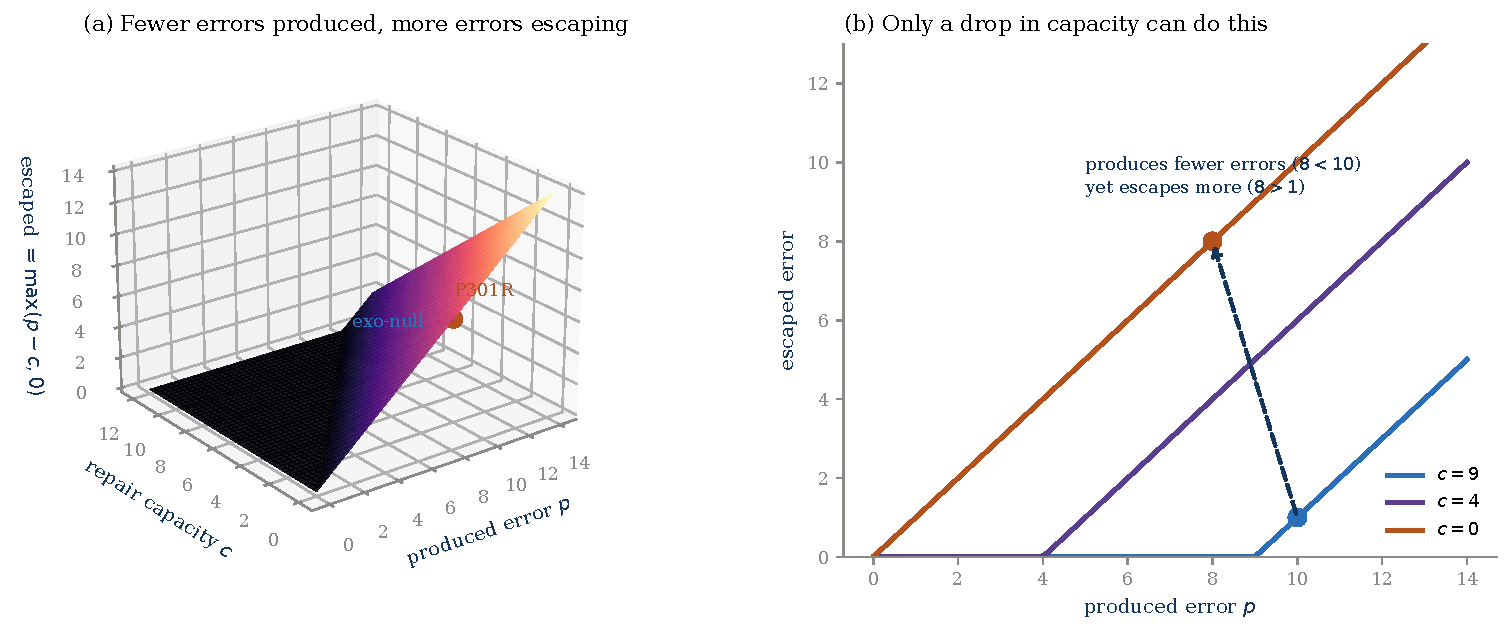
\includegraphics[width=\textwidth]{fig05_repair_reversal.pdf}
  \caption{(a) The escape surface $\mathrm{esc}(p,c) = \max(p-c,0)$. The dashed
  path runs from the exonuclease-null enzyme (high production, intact repair,
  little escaping) to the variant (lower production, no repair capacity, much
  escaping). The path must descend in $c$ --- that is Theorem~\ref{thm:forced}.
  (b) Sections at fixed capacity. Along any single curve the ordering is
  preserved (Theorem~\ref{thm:norev}); the reversal is only possible by moving
  between curves.}
  \label{fig:reversal}
\end{figure}

\subsection{What the model does not settle}

Theorem~\ref{thm:forced} says the capacity differs. It does not say why, and four
mechanisms remain compatible with everything above:

\begin{enumerate}[leftmargin=*,itemsep=1pt]
  \item \textbf{Titration} --- the variant generates lesions that occupy MMR, exhausting it.
  \item \textbf{Interference} --- the variant physically impedes MMR recognition at the fork.
  \item \textbf{Substrate invisibility} --- the variant's errors are of a kind MMR does not see.
  \item \textbf{Loss of extrinsic proofreading} --- the errors are ordinarily
        removed not by MMR but by the exonuclease of polymerase~$\delta$ acting
        in \emph{trans}, and the variant denies them to it. Bulock
        \emph{et al.}\ (2020) show that both MMR and Pol~$\delta$ proofreading are
        required to keep \texttt{pol2-P301R} cells viable, so $c$ in
        Assumption~\ref{model:channel} is lumping together at least two distinct
        repair routes. The model cannot distinguish them, and the book should not
        pretend otherwise.
\end{enumerate}

There is also a constraint that any of these must respect, and it is the reason
this section stops short of a mechanism. The double mutant
\texttt{pol2-P301R msh6$\Delta$} is synthetic lethal --- Xing \emph{et al.}\ (2019)
establish this by tetrad analysis, and report that the double mutants divide into
microcolonies before stopping, the signature of replication error catastrophe ---
whereas \texttt{pol2-4 msh6$\Delta$} is viable. If \texttt{P301R} had already
abolished MMR function, deleting \texttt{MSH6} would add nothing and the double
mutant should be no worse than the single. It is worse. So MMR is still doing
real work on \texttt{P301R} errors, and $c_{\mathrm{mut}} > 0$: the capacity is
reduced, not eliminated.

A student should hold that tension rather than resolve it prematurely. The
textbook's job here is to say exactly how far the evidence reaches.

\begin{worked}[5.1: reading the synthetic lethality as a bound]
\textbf{Problem.} Express the synthetic-lethality observation as a constraint on
$c_{\mathrm{mut}}$ within Assumption~\ref{model:channel}.

\textbf{Solution.} If $c_{\mathrm{mut}} = 0$ the variant already escapes its full
production, $\mathrm{esc}(p_{\mathrm{mut}}, 0) = p_{\mathrm{mut}}$, and removing
\texttt{MSH6} cannot increase it --- there is nothing left to remove. The observed
further deterioration therefore requires $c_{\mathrm{mut}} > 0$.

Combining with Theorem~\ref{thm:forced}: $0 < c_{\mathrm{mut}} < c_{\mathrm{null}}$.
The variant reduces repair capacity without abolishing it. Note that this is a
genuine two-sided bound obtained from two qualitative observations, with no rates
fitted --- an illustration of how much can be extracted from inequalities alone.
\end{worked}

\begin{exercise}
Verify Theorem~\ref{thm:norev} directly for $p_{\mathrm{mut}} = 3$,
$p_{\mathrm{null}} = 7$ and each of $c = 0, 5, 9$. Identify which case is
saturated and which is not.
\end{exercise}

\begin{exercise}
Replace the hard threshold \eqref{eq:escaped} with the Michaelis--Menten form
$\mathrm{esc}(p,c) = p^2/(p + c)$. Show that Theorem~\ref{thm:norev} still holds,
i.e.\ that $\mathrm{esc}$ is non-decreasing in $p$ at fixed $c$ and
non-increasing in $c$ at fixed $p$. What does this tell you about how much the
conclusion depends on the caricature?
\end{exercise}

\begin{exercise}
Design an experiment that would distinguish titration from interference. (Hint:
titration should depend on the \emph{load} of errors produced, interference on
the presence of the variant protein. Consider a catalytically inactive
\texttt{P301R} that still assembles at the fork.)
\end{exercise}

\begin{exercise}[(harder)]
The decisive experiment for the mechanism is a rate measurement in a
\emph{hypomorphic} MMR background rather than a null one. Explain, using
\eqref{eq:escaped}, why a null background ($c = 0$ for both enzymes) cannot
separate the hypotheses, and what a partial reduction in $c$ would reveal.
\end{exercise}

\begin{exercise}[(harder)]
Remark~\ref{rem:transport} argues that a hyperactive polymerase could raise
$p_{\mathrm{mut}}$ in vivo without changing the per-nucleotide error rate the
purified assay reports. Write Assumption~\ref{model:channel} with $p$ expressed
as (errors per nucleotide) $\times$ (nucleotides synthesised per genome), and
show that Theorem~\ref{thm:forced}'s hypothesis constrains the \emph{product} and
not the first factor alone. Then state which of the two factors each of the two
experiments of Section~\ref{sec:refutation} actually measures.
\end{exercise}

\begin{ledger}
\textbf{Measured:} the two comparisons inherited from
Section~\ref{sec:refutation}; the viability of \texttt{pol2-4 msh6$\Delta$} and
the synthetic lethality of \texttt{pol2-P301R msh6$\Delta$} (Xing \emph{et al.},
2019, tetrad analysis); the joint requirement for MMR and Pol~$\delta$
proofreading (Bulock \emph{et al.}, 2020). \\
\textbf{Assumed:} Assumption~\ref{model:channel} --- that repair acts as a
capacity-limited subtraction. The hard threshold is a caricature; Exercise~5.2
shows the qualitative conclusion survives a smooth alternative. \emph{And}, as
Remark~\ref{rem:transport} sets out, that the in vitro ordering
$p_{\mathrm{mut}} \le p_{\mathrm{null}}$ still holds in a cell. Xing
\emph{et al.}'s hyperactivity result gives a concrete reason it might not, and
nothing in this book rules that out. The capacity drop is therefore
\emph{conditionally} forced, and the condition is a modelling assumption rather
than a measurement. \\
\textbf{Proved:} Theorems~\ref{thm:norev} and~\ref{thm:forced}
(\lean{no_reversal_at_fixed_capacity}, \lean{reversal_forces_capacity_drop}),
with a non-vacuity witness and two controls. Gate: $11$ of $11$ clean. What is
proved is the implication; the ledger line above is why the implication's
antecedent is not itself established. \\
\textbf{Open:} which of titration, interference, substrate invisibility or loss
of extrinsic Pol~$\delta$ proofreading operates --- and, prior to that, whether
production is ordered the same way in vivo as in vitro. No measurement reported
here distinguishes any of them, and the hypomorphic experiment of
Exercise~5.4 has not been done. A measurement of error production per replicated
genome, rather than per nucleotide incorporated, would settle the transport
question and has not been made.
\end{ledger}
